%% LyX 2.2.3 created this file.  For more info, see http://www.lyx.org/.
%% Do not edit unless you really know what you are doing.
\documentclass[12pt,english]{article}
\usepackage[osf]{mathpazo}
\renewcommand{\sfdefault}{lmss}
\renewcommand{\ttdefault}{lmtt}
\usepackage[T1]{fontenc}
\usepackage[latin9]{inputenc}
\usepackage[paperwidth=30cm,paperheight=35cm]{geometry}
\geometry{verbose,tmargin=3cm,bmargin=3cm}
\setlength{\parindent}{0bp}
\usepackage{amsmath}
\usepackage{amssymb}

\makeatletter

%%%%%%%%%%%%%%%%%%%%%%%%%%%%%% LyX specific LaTeX commands.
%% Because html converters don't know tabularnewline
\providecommand{\tabularnewline}{\\}

%%%%%%%%%%%%%%%%%%%%%%%%%%%%%% User specified LaTeX commands.
\usepackage{tikz}
\usetikzlibrary{matrix,arrows,decorations.pathmorphing}
\usetikzlibrary{shapes.geometric}
\usepackage{tikz-cd}
\usepackage{amsthm}
\theoremstyle{plain}
\newtheorem{theorem}{Theorem}[section]
\newtheorem{lemma}[theorem]{Lemma}
\newtheorem{prop}{Proposition}[section]
\newtheorem*{cor}{Corollary}
\theoremstyle{definition}
\newtheorem{defn}{Definition}[section]
\newtheorem{ex}{Exercise} 
\newtheorem{example}{Example}[section]
\theoremstyle{remark}
\newtheorem*{rem}{Remark}
\newtheorem*{note}{Note}
\newtheorem{case}{Case}
\usepackage{graphicx}
\usepackage{amssymb}
\usepackage{tikz-cd}
\usetikzlibrary{calc,arrows,decorations.pathreplacing}
\tikzset{mydot/.style={circle,fill,inner sep=1.5pt},
commutative diagrams/.cd,
  arrow style=tikz,
  diagrams={>=latex},
}

\usepackage{babel}
\usepackage{hyperref}
\hypersetup{
    colorlinks,
    citecolor=black,
    filecolor=black,
    linkcolor=black,
    urlcolor=black
}
\usepackage{pgfplots}
\usetikzlibrary{decorations.markings}
\pgfplotsset{compat=1.9}

\makeatother

\usepackage{babel}
\begin{document}

\title{An Interesting (Co)chain Complex and its (Co)homology}

\author{Michael Nelson}

\maketitle
\pagebreak{}

\tableofcontents{}

\pagebreak{}

\part*{Part I}

\section{Notations and Preliminary Material}

~~~Throughout this part of the article, we write $K$ to denote
the field $\mathbb{F}_{2}$. We also write $S$ to denote the polynomial
ring $K[x_{1},\dots,x_{n}]$. We fix a (global) monomial ordering
throughout this article (except in the case when we are describing
a concrete example). So if $I$ is an ideal in $S$, then there is
a unique reduced Gr�bner basis of $I$ with respect to this monomial
ordering (see the book ``Ideals, Varieties, and Algorithms: An Introduciton
to Computation Algebraic Geometry and Commutative Algebra'' for details).
When we write ``let $G$ be the reduced Gr�bner basis of $I$'',
it is understood that $G$ is the reduced Gr�bner basis for $I$ with
respect to the fixed monomial order. Let $f$ be a polynomial in $S$
and let $I$ be an ideal in $S$. Since the monomials form a $K$-basis
of $S$, we can express $f$ as a unique sum of monomials: $f=m_{1}+m_{2}+\cdots+m_{r}$.
We shall refer to the monomials $m_{i}$ as \textbf{terms} of $f$.
We use notation $\text{LT}(f)$ to mean the lead term of $f$ with
respect to the fixed monomial ordering. We also use the notation $\text{LT}(I)$
to denote the monomial ideal generated by the set of all $\text{LT}(f)$
such that $f$ is in $I$. 

\subsection{Homological Algebra}

~~~Let $R$ be a ring. A \textbf{chain complex} $\mathbf{A}_{\bullet}=(A_{\bullet},d_{\bullet})$
\textbf{over} $R$ is a sequence of $R$-modules $A_{i}$ and morphisms
$d_{i}:A_{i}\to A_{i-1}$ \begin{equation}\label{diagramA}\begin{tikzcd} \mathbf{A} _{\bullet } := \cdots \arrow[r] & A_{i+1} \arrow[r,"d _{i+1}"] & A_i  \arrow[r," d _i "] & A_{i-1} \arrow[r] & \cdots \end{tikzcd}\end{equation}

such that $d_{i}\circ d_{i+1}=0$ for all $i\in\mathbb{Z}$. The condition
$d_{i}\circ d_{i+1}=0$ is equivalent to the condition $\text{Ker}(d_{i})\supset\text{Im}(d_{i+1})$.
With this in mind, we define the \textbf{$i$th} \textbf{homology
of the chain complex} $\mathbf{\mathbf{A}_{\bullet}}$ to be 
\[
H_{i}(\mathbf{\mathbf{A}_{\bullet}}):=\text{Ker}(d_{i})/\text{Im}(d_{i+1}).
\]
To clean notation, we usually omit the subscript $i$ in $d_{i}$
and just write $d$, as long as there is no source for confusion.
We also refer to the map $d$ as the \textbf{differential}. 

~~~A \textbf{chain map} between two chain complexes $\mathbf{A}_{\bullet}=(A_{\bullet},d_{\bullet})$
and $\mathbf{A}_{\bullet}'=(A'_{\bullet},d'_{\bullet})$ over $R$
is a sequence $\varphi_{\bullet}$ of $R$-module homomorphisms $\varphi_{i}:A_{i}\to A'_{i}$
such that $d_{i}\varphi_{i-1}=\varphi_{i}d_{i-1}'$ for all $i$.
It then follows that a chain map gives rise to map an induced map
on homology $H_{i}(\mathbf{A}_{\bullet})\to H_{i}(\mathbf{A}_{\bullet}')$. 

~~~The dual notion to a chain complex is a \textbf{cochain complex
}$\mathbf{A}^{\bullet}=(A^{\bullet},\delta^{\bullet})$ over $R$.
It is just a chain complex, except we label things differently. Namely,
we replace subscripts with superscripts. Also, the maps $\delta^{i}$
increase the superscript rather than decrease it: $\delta^{i}:S^{i}\to S^{i+1}$.
As with the differential, we usually omit the superscript $i$ in
$\delta^{i}$ and just write $\delta$. We also refer to the $\delta$
as the \textbf{codifferential}. We define the \textbf{$i$th} \textbf{cohomology
of the cochain complex} $\mathbf{\mathbf{A}^{\bullet}}$ to be 
\[
H^{i}(\mathbf{\mathbf{A}}^{\bullet}):=\text{Ker}(\delta^{i+1})/\text{Im}(\delta^{i}).
\]

It may seem as if we gain nothing new with cochain complexes, but,
as we will see, there are some interesting mathematical objects which,
simultaneously, have a compatible chain and cochain complex. 

\subsection{Gr�bner Basis}

~~~Let $I$ be a homogeneous ideal in the polynomial ring $S$,
and let $G=\{g_{1},g_{2}\dots,g_{r}\}$ be the reduced Gr�bner basis
for $I$. Recall that every polynomial $f\in K[x_{1},\dots,x_{n}]$
can be written as $f=g+r$, where $g\in I$ and no term of $r$ is
divisible by any element of $\text{LT}(I),$ and, moreover, $g$ and
$r$ are uniquely determined. We use the notation $f^{G}:=r$ and
call this the \textbf{normal form of} $f$ \textbf{with respect to
$I$ }(or simply the \textbf{normal form of $f$ }if the there is
no confusion of the ideal $I$). We also use the notation $\pi(f):=f-f^{G}=g$
(since we are working over a characteristic $2$ field, we can just
write $\pi(f)=f+f^{G}$). It follows from uniqueness of $f^{G}$ and
$f+f^{G}$ that taking the normal form of a polynomial is a $K$-linear
map:
\begin{equation}
c_{1}f_{1}^{G}+c_{2}f_{2}^{G}=(c_{1}f_{1}+c_{2}f_{2})^{G}\qquad\text{for all }c_{1},c_{2}\in K\text{ and }f_{1},f_{2}\in S.\label{eq:Klinearity}
\end{equation}

We will denote this map as $-^{G}$. So $-^{G}$ is the $K$-linear
map which takes $f$ to $f^{G}$.

\subsection{Graded $K$-Algebras and $K$-Modules}

~~~Let $I$ be a homogeneous ideal in the polynomial ring $S$
and let $G=\{g_{1},g_{2}\dots,g_{r}\}$ be the reduced Gr�bner basis
for $I$. Recall that $S$ is a graded $K$-algebra, where the homogeneous
component $S_{i}$ is the $K$-vector space of all homogeneous polynomials
$f\in S$ of degree $i$. By a graded $K$-algebra, we mean there
is a direct sum $S=\bigoplus_{i\geq0}S_{i}$ where $S_{i}S_{j}\subseteq S_{i+j}$
and $S_{0}=K$. Since $I$ is a homogeneous ideal, the ring $S/I$
is also a graded $K$-algebra, where the homogeneous component in
degree $i$ is $(S/I)_{i}:=S_{i}/(I\cap S_{i})$. 

~~~Define $S_{I}:=\text{Span}_{K}(x^{\alpha}\mid x^{\alpha}\notin\langle\text{LT}(I)\rangle)$.
There is an obvious decompostion of $S_{I}$ into $K$-vector spaces
$(S_{I})_{i}$, where $(S_{I})_{i}=\text{Span}_{K}(x^{\alpha}\mid x^{\alpha}\notin\langle\text{LT}(I)\rangle\text{ and }\text{deg}(x^{\alpha})=i)$.
In fact, $S/I$ and $S_{I}$ are isomorphic as graded $K$-algebras.
The isomorphism is given by mapping $\overline{f}\in S/I$ to $f^{G}\in S_{I}$,
where $K$-linearity follows from (\ref{eq:Klinearity}) and $-^{G}$
preserves homogeneity (respects the grading). This makes $S/I$ isomorphic
to $S_{I}$ as graded $K$-modules. Using this isomorphism, we can
carry multiplication from $S/I$ over to $S_{I}$ to turn $S_{I}$
into a graded $K$-algebra: For $f_{1},f_{2}\in S_{I}$, we define
multiplication as
\begin{equation}
f_{1}\cdot f_{2}=(f_{1}f_{2})^{G}\label{eq:SImult}
\end{equation}
Defining multilpication this way makes $S_{I}$ isomorphic to $S/I$
as graded $K$-algebras. For our purposes, it'll be easier to work
with $S_{I}$ rather than $S/I$. 

\begin{example}\label{examplediffalgSI} Consider $S=K[x,y]$ and
$I=\langle xy^{2}+y^{3},x^{3}+x^{2}y\rangle$. Then $G=\{xy^{2}+y^{3},x^{3}+x^{2}y\}$
is the reduced Gr�bner basis with respect to graded reverse lexicographical
order. Thus $\text{LT}(I)=\langle xy^{2},x^{3}\rangle$. Let's do
some computations in $S_{I}$. First, let's write the first few homogeneous
terms of $S_{I}$:
\begin{align*}
(S_{I})_{0} & =K\\
(S_{I})_{1} & =Kx+Ky\\
(S_{I})_{2} & =Kx^{2}+Kxy+Ky^{2}\\
(S_{I})_{3} & =Kx^{2}y+Ky^{3}\\
(S_{I})_{4} & =Ky^{4}\\
(S_{I})_{5} & =Ky^{5}\\
 & \vdots
\end{align*}

Next, we multiply some elements together in $S_{I}$ in the multiplication
table below
\begin{center}
\begin{tabular}{c|ccc}
$\cdot$ & $x$ & $y$ & $y^{3}$\tabularnewline
\hline 
$x^{2}y$ & $y^{4}$ & $y^{4}$ & $y^{6}$\tabularnewline
$x^{2}$ & $x^{2}y$ & $x^{2}y$ & $y^{5}$\tabularnewline
$x$ & $x^{2}$ & $xy$ & $y^{4}$\tabularnewline
\end{tabular}
\par\end{center}

\end{example}

~~~Finally, we briefly mention that $I$ is a graded $S$-module
where the homogeneous component $I_{i}$ is $I_{i}:=I\cap S_{i}$.
By graded $S$-module, we mean there is a direct sum $I=\bigoplus_{i\geq0}I_{i}$
where $S_{i}I_{j}\subseteq I_{i+j}$. In particular, $I$ is a graded
$K$-module, and by this, we simply mean that there is a direct sum
$I=\bigoplus_{i\geq0}I_{i}$ where the $I_{i}$ are $K$-vector spaces. 

\begin{example}\label{example} Consider $S=K[x,y]$ and $I=\langle xy+y^{2},x^{3}\rangle$.
We first use Singular to compute a Gr�bner basis $G$ of $I$ with
respect to graded reverse lexicographical order. We obtain $G=\{g_{1},g_{2},g_{3}\}$.
where $g_{1}=xy+y^{2}$, $g_{2}=x^{3}$, and $g_{3}=y^{4}$. Then
\begin{align*}
I_{0} & =0 & (S/I)_{0} & =K\cdot\overline{1} & (S_{I})_{0} & =K\\
I_{1} & =0 & (S/I)_{1} & =K\overline{x}+K\overline{y} & (S_{I})_{1} & =Kx+Ky\\
I_{2} & =Kg_{1} & (S/I)_{2} & =K\overline{x}^{2}+K\overline{y}^{2} & (S_{I})_{2} & =Kx^{2}+Ky^{2}\\
I_{3} & =Kxg_{1}+Kyg_{1}+Kg_{2} & (S/I)_{3} & =K\overline{y}^{3} & (S_{I})_{3} & =Ky^{3}\\
I_{4} & =S_{4} & (S/I)_{4} & =0 & (S_{I})_{4} & =0\\
 & \vdots &  & \vdots &  & \vdots
\end{align*}

\end{example}

\section{The Chain Complexes $\mathbf{A}_{\bullet}(S)$, $\mathbf{A}_{\bullet}(S_{I})$,
and $\mathbf{A}_{\bullet}(I)$. }

~~~Throughout this section, let $I$ be a homogeneous ideal in
the polynomial ring $S$ and let $G=\{g_{1},g_{2}\dots,g_{r}\}$ be
the reduced gr�bner basis for $I$.

\subsection{Construction of $\mathbf{A}_{\bullet}(S)$}

~~~Let $d_{i}:S_{i}\to S_{i-1}$ be the map given by $d_{i}:=\sum_{j=1}^{n}\partial_{x_{j}}$.
To simplify notation, we often omit the subscript $i$ in $d_{i}$
and write $d$. We shall refer to $d$ as the \textbf{differential}
\textbf{map for $S$ }or simply the \textbf{differential}. This differential
map is clearly $K$-linear, and since we are working over a field
of characteristic $2$, we have $d^{2}=0$: Let $m=x_{1}^{\alpha_{1}}\cdots x_{n}^{\alpha_{n}}$
be a monomial in $S_{i}$, then
\begin{align*}
d^{2}(m) & =\left(\sum_{k=1}^{n}\partial_{x_{k}}\right)^{2}\left(x_{1}^{\alpha_{1}}\cdots x_{n}^{\alpha_{n}}\right)\\
 & =\left(\sum_{k=1}^{n}\partial_{x_{k}}^{2}\right)\left(x_{1}^{\alpha_{1}}\cdots x_{n}^{\alpha_{n}}\right)\\
 & =\sum_{k=1}^{\infty}\alpha_{k}(\alpha_{k}-1)x_{1}^{\alpha_{k}-2}\\
 & =0.
\end{align*}

Thus the differential $d$ gives the graded $K$-algebra $S$ the
structure of a chain complex over $K$, which we denote $\mathbf{A}_{\bullet}(S):=(S_{\bullet},d_{\bullet})$.
We shall denote the $i$th homology of $\mathbf{A}_{\bullet}(S)$
as $H_{i}(S)$. 

\subsection{Construction of $\mathbf{A}_{\bullet}(S_{I})$}

~~~Let $m=x_{1}^{\alpha_{1}}\cdots x_{n}^{\alpha_{n}}$ be a monomial
of degree $i$ in $S$. We denote 
\[
[m]_{o}=\{1\leq\lambda\leq n\mid\alpha_{\lambda}\text{ is odd}\}\qquad\text{and}\qquad[m]_{e}=\{1\leq\mu\leq n\mid\alpha_{\mu}\text{ is even}\}
\]
Using this notation, we can express the differential in another way:
\[
d(m)=\sum_{\lambda\in[m]_{o}}x_{\lambda}^{-1}m.
\]
This makes it clear, for example, that the differential maps $(S_{I})_{i}$
into $(S_{I})_{i-1}$ for all $i$: If $m$ is not in $\text{LT}(I)$,
then every term $x_{\lambda}^{-1}m$ of $d(m)$ is not in $\text{LT}(I)$
either. Thus, the differential $d$ restricts to $S_{I}$ and gives
the graded $K$-algebra $S_{I}$ the structure of a chain complex
over $K$, which we denote $\mathbf{A}_{\bullet}(S_{I}):=((S_{I})_{\bullet},d_{\bullet})$.
We shall also denote the $i$th homology of $\mathbf{A}_{\bullet}(S_{I})$
as $H_{i}(S_{I})$. 

\subsection{Construction of $\mathbf{A}_{\bullet}(I)$}

~~~Our final construction involves the graded $K$-module $I$.
Using the fact that the inclusion map $I_{i}\hookrightarrow S_{i}$
splits $\pi$, we can construct a map $\overline{d}:I_{i}\to I_{i-1}$,
where $\overline{d}(f):=d(f)+d(f)^{G}=\pi(d(f))$ for all $f\in I_{i}$.
The map $\overline{d}$ gives the graded $K$-module $I$ the structure
of a chain complex over $K$, which we denote $\mathbf{A}_{\bullet}(I):=(I{}_{\bullet},\overline{d}_{\bullet})$.
Indeed, for all $f\in I$, we have 
\begin{align*}
\overline{d}(\overline{d}(f)) & =\overline{d}(d(f)+d(f)^{G})\\
 & =d(d(f)+d(f)^{G})+d(d(f)+d(f)^{G})^{G}\\
 & =d(d(f)^{G})+d(d(f)^{G})^{G}\\
 & =d(d(f)^{G})+d(d(f)^{G})\\
 & =0,
\end{align*}
where $d(d(f)^{G})^{G}=d(d(f)^{G})$ since every term in $d(d(f)^{G})$
is not in $I$. We shall also denote the $i$th homology of $\mathbf{A}_{\bullet}(I)$
as $H_{i}(I)$ and we will refer to $\overline{d}$ as the differential
map for\textbf{ $I$ }or, by abuse of notation, simply the differential.

\subsection{Summary}

We provide a summary of our constructions in the table below. 
\begin{center}
\begin{tabular}{c|c|c|c}
Chain Complex & Homogeneous Components & Differential & Homology\tabularnewline
\hline 
\hline 
$\mathbf{A}_{\bullet}(S):=(S_{\bullet},d_{\bullet})$ & $\mathbf{\mathbf{A}_{\bullet}}(S)_{i}:=S_{i}$  & $d:S_{i}\to S_{i-1}$ & $H_{i}(S)$\tabularnewline
\hline 
$\mathbf{A}_{\bullet}(I):=((I)_{\bullet},\overline{d}_{\bullet})$ & $\mathbf{A}_{\bullet}(I)_{i}:=I_{i}$ & $\overline{d}:I_{i}\to I_{i-1}$ & $H_{i}(I)$\tabularnewline
\hline 
$\mathbf{A}_{\bullet}(S_{I}):=((S_{I})_{\bullet},d_{\bullet})$ & $\mathbf{A}_{\bullet}(S_{I})_{i}:=(S_{I})_{i}$ & $d:(S_{I})_{i}\to(S_{I})_{i-1}$ & $H_{i}(S_{I})$\tabularnewline
\end{tabular}
\par\end{center}

\section{Differential Graded Algebras}

\subsection{Differential Graded Algebra Structure on $\mathbf{A}_{\bullet}(S)$}

~~~It turns out that $\mathbf{A}_{\bullet}(S)$ is more than just
a chain complex over $K$, in fact it can be given the structure of
a differential graded algebra over $K$. Let's recall the definition
of what a differential graded algebra over a ring is.

\begin{defn}\label{defn} Let $R$ be a ring. A \textbf{differential
graded algebra over $R$ }is a chain complex $A=(A_{\bullet},d_{\bullet})$
over $R$, together with $R$-bilinear maps $A_{i}\times A_{j}\to A_{i+j}$,
denoted $(a,b)\mapsto ab$, such that the \textbf{Leibniz law }holds:
\begin{equation}
d_{i+j}(ab)=d_{i}(a)b+(-1)^{i}ad_{j}(b).\label{eq:leibniz1}
\end{equation}
for all $a,b\in A$. 

\end{defn}

\begin{rem}\label{rem} To ease notation, we usually drop the subscripts
in (\ref{eq:leibniz1}) as long as there is no source of confusion.
Then using this together with the fact that we are working over a
field of characteristic $2$, we can simplify (\ref{eq:leibniz1})
to 
\[
d(ab)=d(a)b+ad(b).
\]

\end{rem}

~~~Since $S$ is already a graded $K$-algebra, we already have
$K$-bilinear maps $S_{i}\times S_{j}\to S_{i+j}$ (the usual multiplication
map). Leibniz law follows since $d$ is defined in terms of partial
derivatives. We use these bilinear maps together with the differential
$d$ to give $\mathbf{A}_{\bullet}(S)$ the structure of a differential
graded algebra over $K$. 

\subsection{Almost Differential Graded Algebra Structure on $\mathbf{A}_{\bullet}(S_{I})$.}

~~~Let $I$ be a homogeneous ideal in the polynomial ring $S$,
and let $G=\{g_{1},g_{2}\dots,g_{r}\}$ be the reduced gr�bner basis
for $I$. Recall that $S_{I}$ is a graded $K$-algebra. It is natural
wonder if we can give $\mathbf{A}_{\bullet}(S_{I})$ the structure
of a differential graded algebra over $K$ using the $K$-bilinear
maps which come from $S_{I}$. A quick counterexample shows that this
is not necessarily the case: Consider $S=K[x]$ and $I=\langle x^{5}\rangle$.
Then
\begin{align*}
d(x\cdot x^{4}) & =d((x^{5})^{G})\\
 & =d(0)\\
 & =0,
\end{align*}
but 
\begin{align*}
d(x)\cdot x^{4}+x\cdot d(x^{4}) & =1\cdot x^{4}+x\cdot0\\
 & =(x^{4})^{G}+0^{G}\\
 & =x^{4},
\end{align*}
so $d(x\cdot x^{5})\neq d(x)\cdot x^{4}+x\cdot d(x^{4})$. 

~~~The next proposition tells us precisely when we can give $\mathbf{A}_{\bullet}(S_{I})$
the structure of a differential graded algebra over $K$ using the
$K$-bilinear maps which come from $S_{I}$.

\begin{prop}\label{propdgalgebrasi} Let $I$ be a homogeneous ideal
in the polynomial ring $S$ and let $G=\{g_{1},g_{2}\dots,g_{r}\}$
be the reduced Gr�bner basis for $I$. Suppose that $d(g_{i})=0$
for all $g_{i}$ in $G$. Then $d(f^{G})=d(f)^{G}$ for all $f\in S$.
In particular, this implies that $\mathbf{A}_{\bullet}(S_{I})$ can
be given the structure of a differential graded algebra over $K$
using the $K$-bilinear maps in (\ref{eq:SImult}). Conversely, suppose
$\mathbf{A}_{\bullet}(S_{I})$ can be given the structure of a differential
graded algebra over $K$ using the bilinear maps in (\ref{eq:SImult}).
Then $d(g_{i})=0$ for all $g_{i}$ in $G$. \end{prop}

\begin{proof} First we show that $d(f^{G})=d(f)^{G}$ for all $f\in S$.
Let $f\in S$. From the division algorithm, we have $f=g_{1}q_{1}+\cdots+g_{r}q_{r}+f^{G}$
for some $q_{1},\dots,q_{r}\in S$. Thus 
\begin{align*}
d(f) & =d(g_{1}q_{1}+\cdots+g_{r}q_{r}+f^{G})\\
 & =d(g_{1}q_{1})+\cdots+d(g_{r}q_{r})+d(f^{G})\\
 & =g_{1}d(q_{1})+\cdots+g_{r}d(q_{r})+d(f^{G}).
\end{align*}
Since $g_{1}d(h_{1})+\cdots+g_{r}d(h_{r})\in I$ and no term of $d(f^{G})$
is divisible by any element of $\text{LT}(I)$, it follows from uniqueness
of normal forms that $d(f^{G})=d(f)^{G}$. 

~~~Now we show that this implies that $\mathbf{A}_{\bullet}(S_{I})$
can be given the structure of a differential graded algebra over $K$
using the $K$-bilinear maps in (\ref{eq:SImult}). Let $f_{1},f_{2}\in S_{I}$.
Then 
\begin{align*}
d(f_{1}\cdot f_{2}) & =d((f_{1}f_{2})^{G})\\
 & =(d(f_{1}f_{2}))^{G}\\
 & =(d(f_{1})f_{2}+f_{1}d(f_{2}))^{G}\\
 & =(d(f_{1})f_{2})^{G}+(f_{1}d(f_{2}))^{G}\\
 & =d(f_{1})\cdot f_{2}+f_{1}\cdot d(f_{2}).
\end{align*}

~~Now we prove the converse. Assume $\mathbf{A}_{\bullet}(S_{I})$
can be given the structure of a differential graded algebra over $K$
using the $K$-bilinear maps in (\ref{eq:SImult}). Let $g\in G$.
We may assume $g$ is not a constant (otherwise we'd clearly have
$d(g)=0$). Let $m$ be the lead term of $g$. Since $g$ is not a
constant, there exists some $x_{\lambda}$ such that $x_{\lambda}$
divides $m$. Then on the one hand, we have
\begin{align*}
d(x_{\lambda}\cdot x_{\lambda}^{-1}m) & =d(m^{G})\\
 & =d(g+m)\\
 & =d(g)+d(m),
\end{align*}
since $m^{G}=g+m$. On the other hand, we have 
\begin{align*}
d(x_{\lambda})\cdot x_{\lambda}^{-1}m+x_{\lambda}\cdot d(x_{\lambda}^{-1}m) & =(x_{\lambda}^{-1}m)^{G}+(x_{\lambda}d(x_{\lambda}^{-1}m))^{G}\\
 & =x_{\lambda}^{-1}m+(x_{\lambda}d(x_{\lambda}^{-1}m))^{G}\\
 & =x_{\lambda}^{-1}m+(x_{\lambda}(x_{\lambda}^{-2}m+x_{\lambda}^{-1}d(m)))^{G}\\
 & =x_{\lambda}^{-1}m+(x_{\lambda}^{-1}m+d(m))^{G}\\
 & =x_{\lambda}^{-1}m+(x_{\lambda}^{-1}m)^{G}+d(m)^{G}\\
 & =x_{\lambda}^{-1}m+x_{\lambda}^{-1}m+d(m)^{G}\\
 & =d(m),
\end{align*}

since $(x_{\lambda}^{-1}m)^{G}=x_{\lambda}^{-1}m$ and $d(m)^{G}=d(m)$
(every term of $d(m)$ does not lie in $\langle\text{LT}(G)\rangle$).
Since $\mathbf{A}_{\bullet}(S_{I})$ can be given the structure of
a differential graded algebra over $K$ using the $K$-bilinear maps
in (\ref{eq:SImult}), we must have $d(g)=0$. Since $g$ was arbitrarily
chosen, we have $d(g)=0$ for all $g\in G$. \end{proof}

\begin{rem}\label{rem} We should note that the identity $x_{\lambda}d(x_{\lambda}^{-1}m)=x_{\lambda}(x_{\lambda}^{-2}m+x_{\lambda}^{-1}d(m))=x_{\lambda}^{-1}m+d(m)$
follows since $d$ satisfies Leibniz law not just in $S$, but also
in $S[x_{1}^{-1},\dots,x_{n}^{-1}]$. This is clear since $d$ is
defined in terms of partial derivatives. \end{rem}

\begin{example}\label{example} Going back to Example~(\ref{examplediffalgSI})
where $S=K[x,y]$, $I=\langle xy^{2}+y^{3},x^{3}+x^{2}y\rangle$,
and $G=\{xy^{2}+y^{3},x^{3}+x^{2}y\}$. We have $d(xy^{2}+y^{3})=d(x^{3}+x^{2}y)=0$.
By Proposition~(\ref{propdgalgebrasi}), $\mathbf{A}_{\bullet}(S_{I})$
is a differential graded algebra over $K$. \end{example}

~~~In this article, we've mainly fixed a (global) monomial ordering
for simplicity. In the next example however, we want to consider two
different (global) monomial orderings: namely we consider graded reverse
lexicographical order with $x>y>z$ and graded reverse lexicographical
order with $y>x>z$.

\begin{example}\label{examplediffalggrob} Consider $S=K[x,y,z]$
and $I=\langle f_{1},f_{2},f_{3}\rangle$ where 
\begin{align*}
f_{1} & =xy+xz+yz\\
f_{2} & =y^{3}+y^{2}z\\
f_{3} & =x^{4}+y^{4}+z^{4}
\end{align*}
Then $d(f_{1})=d(f_{2})=d(f_{3})=0$, but we can't conclude yet that
$\mathbf{A}_{\bullet}(S_{I})$ can be given the structure of a differential
graded algebra over $K$. We first need to compute a Gr�bner basis
with respect to some (global) monomial ordering. We use Singular to
compute the reduced Gr�bner basis $G$ of $I$ with respect to graded
reverse lexicographical order with $x>y>z$. We obtain $G=\{g_{1},g_{2},g_{3},g_{4},g_{5},g_{6},g_{7}\}$
where
\begin{align*}
g_{1} & =xy+xz+yz\\
g_{2} & =y^{3}+y^{2}z\\
g_{3} & =y^{2}z^{2}\\
g_{4} & =x^{4}+y^{4}\\
g_{5} & =xz^{4}+yz^{4}\\
g_{6} & =x^{3}z^{2}+x^{2}z^{3}+yz^{4}+z^{5}\\
g_{7} & =z^{6}.
\end{align*}
One can easily see that $d(g)=0$ for all $g\in G$, and now we can
conclude that $\mathbf{A}_{\bullet}(S_{I})$ can be given the structure
of a differential graded algebra over $K$ using the $K$-bilinear
maps in (\ref{eq:SImult}) obtained from $G$. 

~~~In fact, we could have used a \emph{different }(global) monomial
ordering and obtained it's corresponding reduced Gr�bner basis $G'$,
and we'd still have $d(g')=0$ for all $g'\in G'$. For instance,
we use Singular to compute the reduced Gr�bner basis $G'$ of $I$
with respect to graded reverse lexicographical order with $y>x>z$.
We obtain $G'=\{g'_{1},g'_{2},g'_{3},g'_{4},g'_{5},g'_{6},g'_{7},g'_{8}\}$
where
\begin{align*}
g'_{1} & =yx+yz+xz\\
g'_{2} & =y^{3}+y^{2}z\\
g'_{3} & =y^{2}z^{2}\\
g'_{4} & =x^{4}+y^{4}\\
g'_{5} & =yz^{4}+xz^{4}\\
g'_{6} & =x^{3}z^{2}+x^{2}z^{3}+xz^{4}+z^{5}\\
g'_{7} & =z^{6}.\\
g'_{8} & =x^{2}z^{4}.
\end{align*}

One can easily see that $d(g')=0$ for all $g'\in G'$, and so we
can also conclude that $\mathbf{A}_{\bullet}(S_{I})$ can be given
the structure of a differential graded algebra over $K$ using the
$K$-bilinear maps in (\ref{eq:SImult}) obtained from $G'$. \end{example}

\begin{rem}\label{rem} This example is an instance of a more general
phenomenom, as we will see in the next proposition. \end{rem}

\begin{lemma}\label{lemmadg} Let $I$ be a homogeneous ideal in the
polynomial ring $S$, and let $G=\{g_{1},g_{2},\dots,g_{r}\}$ be
the reduced Gr�bner basis for $I$. Then $d(g)=d(g)^{G}$ for all
$g\in G$. \end{lemma}

\begin{proof} Let $g\in G$. If $d(g)=0$, then clearly we have $d(g)=d(g)^{G}$,
so assume $d(g)\neq0$. We need to prove that $d(g)=d(g)^{G}$. This
is equivalent to saying that no term of $d(g)$ belongs to $\langle\text{LT}(G)\rangle:=\langle\text{LT}(g_{1}),\text{LT}(g_{2}),\dots,\text{LT}(g_{r})\rangle$,
since $G$ is a Gr�bner basis. Every term in of $d(g)$ has the form
$x_{\lambda}^{-1}m$ where $m$ is some term of $g$. It is easy to
see that this term cannot belong to $\text{\ensuremath{\langle}LT}(G)\rangle$.
Indeed, if $x_{\lambda}^{-1}m\in\langle\text{LT}(G)\rangle$, then
$m\in\langle\text{LT}(g_{2}),\dots,\text{LT}(g_{r})\rangle$, and
this contradicts the fact that $G$ is a \emph{reduced }Gr�bner basis.
\end{proof}

\begin{prop}\label{propdiffalggenset} Let $I$ be a homogeneous ideal
in the polynomial ring $S$ and let $G=\{g_{1},g_{2}\dots,g_{r}\}$
be the reduced Gr�bner basis for $I$. Suppose $I$ is generated by
the set of polynomials $F=\{f_{1},f_{2},\dots,f_{s}\}$ such that
$d(f)=0$ for all $f\in F$. Then $d(g)=0$ for all $g\in G$. \end{prop}

\begin{proof} Let $g\in G$. Since $F$ is a generating set for $I$,
we have $g=q_{1}f_{1}+q_{2}f_{2}+\cdots+q_{s}f_{s}$. Therefore
\[
d(g)=d(q_{1}f_{1}+q_{2}f_{2}+\cdots+q_{s}f_{s})=d(q_{1})f_{1}+d(q_{2})f_{2}+\cdots+d(q_{s})f_{s}.
\]
In particular, this implies $d(g)\in I$. Recall that $d(g)\in I$
if and only if $d(g)^{G}=0$. Combining this with Lemma~(\ref{lemmadg}),
we find that $d(g)=d(g)^{G}=0$. \end{proof}

\section{Calculating the Homologies $H_{i}(S_{I})$, $H_{i}(S)$, and $H_{i}(I)$}

\subsubsection{Acyclicity of $\mathbf{A}_{\bullet}(S)$}

We first start with what is essentially a consequence of $\mathbf{A}_{\bullet}(S)$
being a differential graded algebra over $K$. 

\begin{prop}\label{propSisfree} $H_{i}(S)=0$ for all $i\geq0$.
\end{prop}

\begin{proof} Let $f$ be a homogeneous polynomial of degree $i$
such that $d(f)=0$. Then for any $x_{\lambda}\in S_{1}$, we have
\[
d(x_{\lambda}f)=d(x_{\lambda})f+x_{\lambda}d(f)=f.
\]
Therefore, $\text{Ker}(d)=\text{Im}(d)$, which proves the claim.
\end{proof}

\begin{rem}\label{remSIisfreeforspecialG} Let $I$ be a homogeneous
ideal in the polynomial ring $S$, and let $G=\{g_{1},g_{2}\dots,g_{r}\}$
be the reduced Gr�bner basis for $I$. 
\begin{enumerate}
\item Suppose that $d(g_{i})=0$ for all $g_{i}$ in $G$ so that $\mathbf{A}_{\bullet}(S_{I})$
is a differential graded algebra over $K$ by Proposition~(\ref{propdgalgebrasi}).
The same proof shows that $H_{i}(S_{I})=0$ for all $i\geq0$. 
\item Combining Proposition~(\ref{propSisfree}) and Proposition~(\ref{propdgalgebrasi}),
we see that $\mathbf{A}_{\bullet}(S_{I})$ is a differential graded
algebra over $K$ if and only if for each $g\in G$, we have $g=d(f)$
for some $f\in S$. 
\end{enumerate}
\end{rem}

\subsubsection{$H_{i}(I)\protect\cong H_{i-1}(S_{I})$}

\begin{prop}\label{proplongexact} Let $I$ be a homogeneous ideal
in the polynomial ring $S$. Then differential $d$ induces isomorphisms
$H_{i}(I)\cong H_{i-1}(S_{I})$ for all $i>0$. \end{prop}

\begin{proof} First we show that $\overline{d}\pi=\pi d$. For all
$f\in S$, we have
\begin{align*}
\overline{d}(\pi(f)) & =\overline{d}(f+f^{G})\\
 & =d(f+f^{G})+d(f+f^{G})^{G}\\
 & =d(f)+d(f^{G})+d(f)^{G}+d(f^{G})^{G}\\
 & =d(f)+d(f^{G})+d(f)^{G}+d(f^{G})\\
 & =d(f)+d(f)^{G}\\
 & =\pi(d(f)),
\end{align*}

where $d(f^{G})^{G}=d(f^{G})$ because no term in $d(f^{G})$ is in
$\text{LT}(I)$ because no term of $f^{G}$ is in $\text{LT}(I)$. 

~~~It is now easy to see that diagram of $K$-vector spaces below
is commutative with exact rows:

\begin{center}\begin{tikzcd}

& \vdots \arrow[d] & \vdots \arrow[d] & \vdots \arrow[d]

\\

0 \arrow[r] & (S_I )_i \arrow[d, "d"] \arrow[r, hook] & S_i \arrow[d, "d" ] \arrow[r, "\pi "] & I_i \arrow[d, "\overline{d} "] \arrow[r] & 0  

\\

0 \arrow[r] & (S_I )_{i-1} \arrow[r, hook] \arrow[d] & S_{i-1} \arrow[d] \arrow[r, "\pi "] & I_{i-1} \arrow[d] \arrow[r] & 0  

\\ 

& \vdots & \vdots & \vdots




\end{tikzcd}\end{center}

In other words, we have a short exact sequence of chain complexes
over $K$:

\begin{center}\begin{tikzcd} 0 \arrow[r] & A_{\bullet } (S_I )  \arrow[r] & A_{\bullet } (S ) \arrow[r, " \pi "] &  A_{\bullet } (I ) \arrow[r] &  0.  \end{tikzcd}\end{center}

From this, we obtain a long exact sequence in homology, which gives
for each $i>0$, the following short exact sequences:

\begin{center}\begin{tikzcd} 0 = H_i (S) \arrow[r] & H_i (I) \arrow[r, "d"] &  H_{i-1}(S_I ) \arrow[r] & H_{i-1}(S ) = 0.  \end{tikzcd}\end{center}

where $d$ is obtained from the connecting map. In more detail, $d$
maps the element $[f]\in H_{i}(I)$ to the element $[d(f)]\in H_{i-1}(S_{I})$.
\end{proof}

\section{The Cochain Complexes $\mathbf{A}^{\bullet}(S_{I})$, $\mathbf{A}^{\bullet}(S)$,
and $\mathbf{A}^{\bullet}(I)$. }

~~~Throughout this section, let $I$ be a homogeneous ideal in
the polynomial ring $S$ and let $G=\{g_{1},g_{2}\dots,g_{r}\}$ be
the reduced Gr�bner basis for $I$.

\subsection{Duality}

~~~For a $K$-vector space $V$, let $V^{\star}:=\text{Hom}_{K}(V,K)$.
We refer to $V^{\star}$ as the \textbf{dual }of $V$. Recall that
there is a canonical isomorphism $V^{\star\star}\simeq V$. In particular,
we can refer to $V$ as the dual of $V^{\star}$. 

~~~~The duals of $S_{I}$, $S$, and $I$ are all graded $K$-modules,
where the homogeneous components are simply the duals of $(S_{I})_{i}$,
$S_{i}$, and $I_{i}$ respectively. In fact, $S_{I}$, $S/I$, $S$,
and $I$ are all isomorphic as graded $K$-modules to their duals:
To get an isomorphism from $S_{i}$ to $S_{i}^{\star}$, we map the
monomial $x^{\alpha}\in S_{i}$ to the element $\underline{x}^{\alpha}\in S_{i}^{\star}$,
where 
\[
\underline{x}^{\alpha}(x^{\beta})=\begin{cases}
0 & \text{if }\alpha\neq\beta\\
1 & \text{if }\alpha=\beta
\end{cases}
\]
for all monomials $x^{\beta}\in S_{i}$. The isomorphisms $(S_{I})_{i}^{\star}\cong(S_{I})_{i}$
and $I_{i}^{\star}\cong I_{i}$ are induced from this isomorphism.
We often refer to the element $\underline{x}^{\alpha}$ as a monomial
in $S^{\star}$. 

\subsection{Construction of $\mathbf{A}^{\bullet}(S)$}

~~~Recall that $\text{Hom}_{K}(-,K)$ is a contravariant functor,
and so we get a map $d^{\star}:S_{i-1}^{\star}\to S_{i}^{\star}$
which comes from applying $\text{Hom}_{K}(-,K)$ to the differential
$d:S_{i}\to S_{i-1}$. We can describe $d^{\star}$ as follows: Let
$m=x_{1}^{\alpha_{1}}\cdots x_{n}^{\alpha_{n}}$ be a monomial of
degree $i-1$ in $S$. Then
\[
d^{\star}(\underline{m})=\sum_{\mu\in[m]_{e}}\underline{x^{\mu}m}.
\]
~~~Using the isomorphisms described above, we often identify $m$
with $\underline{m}$ and relabel $d^{\star}$ as $\delta$ and call
it the \textbf{codifferential}. Thus, for each monomial $m\in S$,
we have 
\[
\delta(m)=\sum_{\mu\in[m]_{e}}x_{\mu}m.
\]
It is clear that $\delta$ gives $S$ the structure of a cochain complex
over $K$, which we denote $\mathbf{A}^{\bullet}(S):=(S^{\bullet},\delta^{\bullet})$.
We shall denote the $i$th cohomology of $\mathbf{A}^{\bullet}(S)$
as $H^{i}(S)$. 

\begin{rem}\label{rem} The codifferential $\delta$ does \emph{not
}give $\mathbf{A}^{\bullet}(S)$ the structure of a differential graded
algebra over $K$ with respect to the usual multiplication maps. For
instance, consider $S=K[x,y]$. Then $\delta(xy)=0$ but $\delta(x)y+x\delta(y)=x^{2}y+xy^{2}$.
\end{rem}

\subsection{Kronecker Pairing}

~~~When we identify monomials $\underline{x}^{\alpha}$ in $S^{\star}$
with monomials $x^{\alpha}$ in $S_{i}$, we are forgetting the way
monomials in $S_{i}^{\star}$ act on monomials in $S_{i}$. To make
up for this, we introduct a symmetric bilinear form $\langle\cdot,\cdot\rangle$
on $S_{i}$ called the \textbf{Kronecker pairing}. For monomials $x^{\alpha}$
and $x^{\beta}$ in $S_{i}$, we set
\[
\langle x^{\alpha},x^{\beta}\rangle=\underline{x}^{\alpha}(x^{\beta})=\begin{cases}
0 & \text{if }\alpha\neq\beta\\
1 & \text{if }\alpha=\beta
\end{cases}.
\]

Then we extend this linearily to $\langle\cdot,\cdot\rangle:S_{i}\times S_{i}\to K$.
From the way we constructed $\delta$, we have for all $f_{1},f_{2}\in S$,
we have $\langle\delta(f_{1}),f_{2}\rangle=\langle f_{1},d(f_{2})\rangle$. 

\subsection{Construction of $\mathbf{A}^{\bullet}(I)$}

~~~Since $I$ is an ideal, it's easy to see that $\delta$ restricts
to a map $\delta:I_{i-1}\to I_{i}$, and thus gives $I$ the structure
of a cochain complex over $K$, which we denote $\mathbf{A}^{\bullet}(I):=(I^{\bullet},\delta^{\bullet})$.
We shall denote the $i$th cohomology of $\mathbf{A}^{\bullet}(I)$
as $H^{i}(I)$. 

\subsection{Construction of $\mathbf{A}^{\bullet}(S_{I})$ }

~~~Using the fact that the inclusion map $(S_{I})_{i}\hookrightarrow S_{i}$
splits $-^{G}$, we can construct a map $\underline{\delta}:I_{i-1}\to I_{i}$,
where $\underline{\delta}(f):=\delta(f)^{G}$ for all $f\in(S_{I})_{i}$.
The map $\underline{\delta}$ gives the graded $K$-module $S_{I}$
the structure of a cochain complex over $K$, which we denote $\mathbf{A}^{\bullet}(S_{I}):=((S_{I})^{\bullet},\underline{\delta}_{\bullet})$.
We shall also denote the $i$th cohomology of $\mathbf{A}^{\bullet}(S_{I})$
as $H^{i}(S_{I})$ and we will refer to $\overline{\delta}$ as the
codifferential map for\textbf{ $S_{I}$ }or, by abuse of notation,
simply the codifferential.

\subsection{Summary}

~~~The construction of $\mathbf{A}^{\bullet}(S/I)$ is obtained
by using the isomorphism $S/I\cong S_{I}$, but we shall omit the
details for now. Summarizing everything up, we have the following
cochain complexes over $K$:
\begin{center}
\begin{tabular}{c|c|c}
Cochain Complex & Homogeneous Components & Codifferential\tabularnewline
\hline 
\hline 
$\mathbf{A}^{\bullet}(S):=(S^{\bullet},\delta^{\bullet})$ & $\mathbf{\mathbf{A}^{\bullet}}(S)^{i}:=S_{i}$  & $\delta:S_{i-1}\to S_{i}$\tabularnewline
\hline 
$\mathbf{A}^{\bullet}(I):=(I^{\bullet},\delta^{\bullet})$ & $\mathbf{A}^{\bullet}(I)^{i}:=I_{i}$ & $\delta:I_{i-1}\to I_{i}$\tabularnewline
\hline 
$\mathbf{A}^{\bullet}(S_{I}):=(S_{I}^{\bullet},\underline{\delta}^{\bullet})$ & $\mathbf{A}^{\bullet}(S_{I})^{i}:=(S_{I})_{i}$ & $\underline{\delta}:(S_{I})_{i-1}\to(S_{I})_{i}$\tabularnewline
\end{tabular}
\par\end{center}

\subsection{Cup and Cap Product}

~~~We introduce some notation for this subsection. Let $m=x_{1}^{\alpha_{1}}x_{2}^{\alpha_{2}}\cdots x_{n}^{\alpha_{n}}$
be a monomial. If $\alpha_{\lambda}>0$, then $x_{\lambda}\mid m$,
and we say $x_{\lambda}$ is a \textbf{term }of $m$. We say $x_{\lambda}$
is the \textbf{last nonzero term }of $m$ if $x_{\lambda}$ is a term
of $m$ and $x_{\mu}$ is not a term of $m$ for all for all $\mu>\lambda$.
We say $x_{\lambda}$ is the \textbf{first nonzero term }of $m$ if
$x_{\lambda}$ is a term of $m$ and $x_{\mu}$ is not a term of $m$
for all for all $\mu<\lambda$. Recall that $S^{\star}$ is spanned
by elements of the form $\varphi_{m}$, where $m$ is a monomial in
$S$. We shall denote $m^{\star}:=\varphi_{m}$ and say $m^{\star}$
is a monomial in $S^{\star}$. 

\subsubsection{Cup Product}

\begin{defn}\label{defn} Let $m_{1}^{\star}$ and $m_{2}^{\star}$
be monomials $S_{i}^{\star}$ and $S_{j}^{\star}$ respectively. The
\textbf{cup product }of $m_{1}^{\star}$ and $m_{2}^{\star}$ is

\[
m_{1}^{\star}\smile m_{2}^{\star}=\begin{cases}
\frac{(m_{1}m_{2})^{\star}}{x_{\lambda}} & \text{if }x_{\lambda}\text{ is the last nonzero term in }m_{1}\text{ and the first nonzero term in }m_{2}\\
0 & \text{otherwise}
\end{cases}
\]

This extends to a linear map $\smile:S_{i}^{\star}\times S_{j}^{\star}\to S_{i+j-1}^{\star}$
which we call the cup product. \end{defn}

\begin{rem}\label{rem} Note that $(m_{1}m_{2})^{\star}\neq m_{1}^{\star}m_{2}^{\star}$.
\end{rem}

\subsubsection{Cap Product}

\begin{defn}\label{defn} Let $m_{1}^{\star}$ and $m_{2}$ be monomials
$S_{i}^{\star}$ and $S_{j}$ respectively. The \textbf{cap product
}of $m_{1}^{\star}$ and $m_{2}$ is
\[
m_{1}^{\star}\frown m_{2}=\begin{cases}
x_{\lambda}\frac{m_{2}}{m_{1}} & \text{if }m_{1}\mid m_{2},\text{ }x_{\lambda}\text{ is the last nonzero term in }m_{1}\text{ and }x_{\lambda}\text{ is the first nonzero term in }\frac{x_{\lambda}m_{2}}{m_{1}}.\\
0 & \text{otherwise}
\end{cases}
\]
The cap product extends linearly to a map $\frown:S_{i}^{\star}\times S_{j}\to S_{i-j+1}$.
\end{defn}

\section{Topological Interpretation of $H_{i}(S_{I})$ and $H^{i}(S_{I})$ }

~~~Let $I$ be a homogeneous ideal in the polynomial ring $S$
and let $G$ be the reduced Gr�bner basis of $I$. An important observation
is that $H_{i}(S_{\text{LT}(I)})\cong H_{i}(S_{I})$. The reason is
because $\mathbf{A}_{\bullet}(S_{I})$ and $\mathbf{A}_{\bullet}(S_{\text{LT}(I)})$
are clearly isomorphic as chain complexes over $K$, and so they have
the same homology. What's interesting is that $S_{I}$ and $S_{\text{LT}(I)}$
are usually not isomorphic as $K$-algebras. This has important consequences.
For instance, consider Example~(\ref{examplediffalgSI}) where $S=K[x,y]$,
$I=\langle xy^{2}+y^{3},x^{3}+x^{2}y\rangle$, and $G=\{xy^{2}+y^{3},x^{3}+x^{2}y\}$.
In this case, $\text{LT}(I)=\langle xy^{2},x^{3}\rangle$ and $S_{\text{LT}(I)}$
is not a differential graded algebra over $K$. On the other hand,
since $d(xy^{2}+y^{3})=d(x^{3}+x^{2}y)=0$, we know that $\mathbf{A}_{\bullet}(S_{I})$
is a differential graded algebra over $K$. By Remark~(\ref{remSIisfreeforspecialG}),
it follows that $H_{i}(S_{I})=0$ for all $i\geq0$. But this implies
that $H_{i}(S_{\text{LT}(I)})=0$ for all $i\geq0$. 

~~~Now we want to give a topological interpretation of $H_{i}(S_{I})$.
Since $H_{i}(S_{\text{LT}(I)})\cong H_{i}(S_{I})$, we might as well
assume that $I$ is in fact a monomial ideal. However, to get things
started, we will first consider the case where $I$ is a \textbf{squarefree
}monomial ideal. A \textbf{squarefree monomial }in $S$ is a monomial
$m=x_{1}^{\alpha_{1}}\cdots x_{n}^{\alpha_{n}}$ in $S$ such that
for all $1\leq j\leq n$, either $\alpha_{j}=0$ or $\alpha_{j}=1$.
Thus, a squarefree monomial in $S$ looks like $x_{j_{1}}\cdots x_{j_{k}}$
where $1\leq j_{1}<\cdots<j_{k}\leq n$. We say an ideal $I$ is a
\textbf{squarefree} ideal if it is generated by squarefree monomials.
After we give a topological interpetation to $H_{i}(S_{I})$ where
$I$ is squarefree, we will then consider the case where $I$ is an
arbitary monomial ideal. 

\subsection{Simplicial Complexes }

~~~Let $\mathbf{n}$ denote the set $\{1,2,\dots,n\}$. An (abstract)
\textbf{simplicial complex $\Delta$ }on $\mathbf{n}$ is a collection
of subsets of $\mathbf{n}$ such that
\begin{enumerate}
\item The simplicial complex $\Delta$ contains all singletons: $\{i\}\in\Delta$
for all $i=1,2,\dots,n$.
\item The simplicial complex $\Delta$ is closed under containment: if $\sigma\subseteq\mathbf{n}$
and $\sigma\supset\tau$, then $\tau\in\Delta$. 
\end{enumerate}
We frequently identify $\{1,\dots,n\}$ with the variables $\{x_{1},\dots,x_{n}\}$.
An element of a simplicial complex is called a \textbf{face }or \textbf{simplex}.
A simplex $\sigma\in\Delta$ of cardinality $i+1$ is called an $i$-dimensional
face or an $i$-face of $\Delta$. The empty set $\emptyset$, is
the unique face of dimension $-1$, as long as $\Delta$ is not the
\textbf{void complex }$\{\}$ consisting of no subsets of $\{1,\dots,n\}$.
The \textbf{dimension }of $\Delta$, denoted $\text{dim}(\Delta)$,
is defined to be the maximum of the dimensions of its faces (or $-\infty$
if $\Delta=\{\}$). 

\begin{example}\label{examplesimplicialcomplex} The simplicial complex
$\Delta$ on $\{1,2,3,4,5\}$ consisting of all subsets of $\{1,2,3\}$,
$\{2,4\}$, $\{3,4\}$, and $\{5\}$ is pictured below

\begin{center}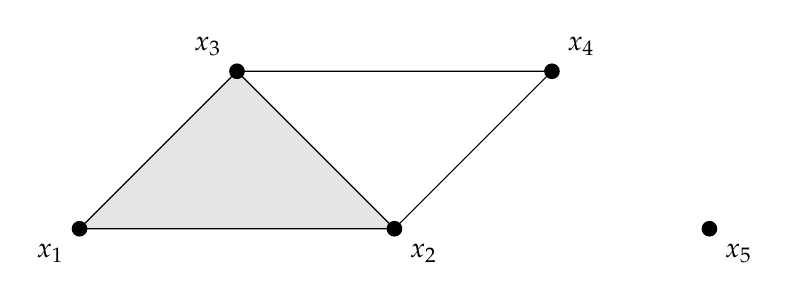
\begin{tikzpicture}

\draw[fill=gray!20] (0,0) -- (2,2) -- (4,0)-- (0,0);
\draw (2,2) -- (6,2) -- (4,0);

\node[circle, fill=black, inner sep=2pt, label=below left:$x_1 $] (a) at (0,0) {};
\node[circle, fill=black, inner sep=2pt, label=above left:$x_3 $] (b) at (2,2) {};
\node[circle, fill=black, inner sep=2pt, label=below right:$x_2 $] (c) at (4,0) {};
\node[circle, fill=black, inner sep=2pt, label=above right:$x_4 $] (c) at (6,2) {};
\node[circle, fill=black, inner sep=2pt, label=below right:$x_5 $] (c) at (8,0) {};




\end{tikzpicture} \end{center}

Note that $\Delta$ is completely specified by its \textbf{facets},
or maximal faces, by definition of the simplicial complex. 

\end{example} 

~~~Let $\Delta$ be a simplicial complex on $\{1,\dots,n\}$. For
$i\in\mathbb{Z}$, let $F_{i}(\Delta)$ be the set of $i$-dimensional
faces of $\Delta$, and let $K^{F_{i}(\Delta)}$ be a $K$-vector
space whose basis elements $e_{\sigma}$ correspond to the $i$-faces
$\sigma\in F_{i}(\Delta)$. The (\textbf{augmented }or \textbf{reduced})
\textbf{chain complex of} $\Delta$ \textbf{over $K$ }is the complex 

\begin{center}\begin{tikzcd} \widetilde{\mathcal{C}}_{\bullet } (\Delta ; K): &  0  & K^{F_{-1} (\Delta ) } \arrow[l] & \cdots \arrow[l, "\partial _{0} ", swap]  & K^{F_{i-1} (\Delta ) } \arrow[l, "\partial _{i-1} ", swap] &   K^{F_{i} (\Delta ) } \arrow[l, "\partial _{i} ", swap] & \cdots  \arrow[l, "\partial _{i+1} ", swap] &  K^{F_{n-1} (\Delta ) } \arrow[l, "\partial _{n-1} ", swap] & 0 \arrow[l] \end{tikzcd}\end{center} 

where for an $i$-face $\sigma$, 
\[
\partial_{i}(e_{\sigma})=\sum_{j\in\sigma}\text{sign}(j,\sigma)e_{\sigma\backslash\{j\}}.
\]
Here $\text{sign}(j,\sigma)=(-1)^{r-1}$ if $j$ is the $r$th element
of the set $\sigma$, written in increasing order (since we are working
over a characteristic $2$ filed though, we can drop the sign all
together and simply write $\partial_{i}(e_{\sigma})=\sum_{j\in\sigma}e_{\sigma\backslash\{j\}}$).
For $i\in\mathbb{Z}$, we define the $i$\textbf{th reduced homology
}of $\Delta$ over $K$ as 
\[
\widetilde{H}_{i}(\Delta,K):=\text{Ker}(\partial_{i})/\text{Im}(\partial_{i+1}).
\]

In particular, $\widetilde{H}_{n-1}(\Delta;K)=\text{Ker}(\partial_{n-1})$
and $\widetilde{H}_{i}(\Delta;K)=0$ for $i<0$ or $n-1<i$, unless
$\Delta=\{\emptyset\}$, in which case $\widetilde{H}_{-1}(\Delta;K)\cong K$
and $\widetilde{H}_{i}(\Delta;K)=0$ for $i\geq0$. The dimension
of $\widetilde{H}_{0}(\Delta;K)$ as a $K$-vector space is one less
than the number of connected components of $\Delta$. Elements of
$\text{Ker}(\partial_{i})$ are called $i$\textbf{-cycles }and elements
of $\text{Im}(\partial_{i+1})$ are called $i$\textbf{-boundaries}. 

\begin{example}\label{example} For $\Delta$ as in Example~(\ref{examplesimplicialcomplex}),
we have 
\begin{align*}
F_{2}(\Delta) & =\{\{1,2,3\}\}\\
F_{1}(\Delta) & =\{\{1,2\},\{1,3\},\{2,3\},\{2,4\},\{3,4\}\}\\
F_{0}(\Delta) & =\{\{1\},\{2\},\{3\},\{4\},\{5\}\}\\
F_{-1}(\Delta) & =\{\emptyset\}
\end{align*}

Choosing bases for the $K^{F_{i}(\Delta)}$ as suggested by the ordering
of the faces listed above, the chain complex for $\Delta$ becomes
\begin{center}\begin{tikzcd}[ampersand replacement=\&] 

0 \& K \arrow[l] \& \& \&  K^5 \arrow[swap]{lll}{\begin{pmatrix} 1 & 1 & 1 & 1 & 1 \end{pmatrix} } \& \& \& \&   K^5 \arrow[swap]{llll}{ \begin{pmatrix} 1 & 1 & 0 & 0 & 0 \\ 1 & 0 & 1 & 1 & 0 \\ 0 & 1 & 1 & 0 & 1  \\ 0 & 0 & 0 & 1 & 1 \\ 0 & 0 & 0 & 0 & 0 \end{pmatrix} } \& \& K \arrow[swap]{ll}{\begin{pmatrix} 1 \\ 1 \\ 1 \\ 0 \\ 0 \end{pmatrix} } \& 0 \arrow[l]



\end{tikzcd}\end{center}

For example, $\partial_{2}(e_{\{1,2,3\}})=e_{\{2,3\}}+e_{\{1,3\}}+e_{\{1,2\}}$,
which we identify with the vector $(1,1,1,0,0)$. The mapping $\partial_{1}$
has rank $3$, so $\widetilde{H}_{0}(\Delta;K)\cong\widetilde{H}_{1}(\Delta;K)\cong K$
and the other homology groups are $0$. Geometrically, $\widetilde{H}_{0}(\Delta;K)$
is nontrivial since $\Delta$ is disconnected and $\widetilde{H}_{1}(\Delta;K)$
is nontrivial since $\Delta$ contains a triangle which is not the
boundary of an element of $\Delta$. \end{example} 

\subsection{Squarefree Monomials and Stanley-Reisner Ring}

~~~There is a nice way of assigning a simplices to a squarefree
monomials: Given a squarefree monomial $x_{j_{1}}\cdots x_{j_{k}}$,
we form the $(k-1)$-simplex whose vertices are labeled $x_{j_{s}}$,
edges with boundary vertices $x_{j_{s}}$ and $x_{j_{t}}$ are labeled
$x_{j_{s}}x_{j_{t}}$, and so on. Under this correspondence, the usual
boundary map defined on simplices precisely matches the differential
$d$ acting on monomials:

\begin{center}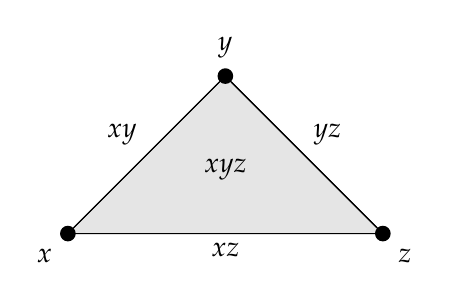
\begin{tikzpicture}

\draw[fill=gray!20] (0,0) -- (2,2) -- (4,0)-- (0,0);

\node[circle, fill=black, inner sep=2pt, label=below left:$x $] (a) at (0,0) {};
\node[circle, fill=black, inner sep=2pt, label=above :$y $] (b) at (2,2) {};
\node[circle, fill=black, inner sep=2pt, label=below right:$z $] (c) at (4,0) {};


\draw[] (a) -- (b) node [midway, above left] {$ xy $};
\draw[] (b) -- (c) node [midway, above right] {$ yz $};
\draw[] (c) -- (a) node [midway, below ] {$ xz $};

\node[label=below:$xyz$] (f) at (2,1.2) {};




\end{tikzpicture} \end{center}

\subsubsection{Stanley-Reisner Ring}

\begin{defn}\label{defn} Let $\Delta$ be a simplicial complex on
$\{1,\dots,n\}$. We denote $I_{\Delta}$ to be the ideal of nonfaces
of $\Delta$: $I_{\Delta}$ is generated by the squarefree monomials
$x_{j_{1}}\cdots x_{j_{k}}$ such that $\{j_{1},\dots,j_{k}\}\notin\Delta$.
We define the \textbf{Stanley-Reisner ring }$K[\Delta]$ of the simplicial
complex $\Delta$ to be the $K$-algebra $K[\Delta]:=S/I_{\Delta}$.
\end{defn}

\begin{rem}\label{rem} The correspondence between simplicial complexes
and squarefree ideals is inclusion reversing: if $\Delta$ and $\Delta'$
are simplicial complexes on the same vertex set, then $\Delta\subset\Delta'$
if and only if $I_{\Delta'}\subset I_{\Delta}$. \end{rem}

\begin{example}\label{example} Consider $S=K[x_{1},x_{2},x_{3},x_{4},x_{5}]$
and $I_{\Delta}=\langle x_{1}x_{4},x_{1}x_{5},x_{2}x_{5},x_{2}x_{3}x_{4},x_{3}x_{5},x_{4}x_{5}\rangle$.
Then $S/I_{\Delta}$ is the Stanley-Reisner ring of the simplex $\Delta$
given in Example~(\ref{examplesimplicialcomplex}). 

~~~Now let $I_{\Delta}^{\text{sq}}=\langle I_{\Delta},x_{1}^{2},x_{2}^{2},x_{3}^{2},x_{4}^{2},x_{5}^{2}\rangle$.
From the correspondence between squarefree monomials and simplices,
we obtain an isomorphism of chain complexes over $K$ from $\widetilde{C}_{\bullet}(\Delta;K)$
to $\mathbf{A}_{\bullet}(S_{I_{\Delta}^{\text{sq}}})$. Let's write
down each homogeneous piece side by side:
\begin{align*}
K^{F_{2}(\Delta)} & =Ke_{\{1,2,3\}} & (S_{I_{\Delta}^{\text{sq}}})_{_{3}} & =Kx_{1}x_{2}x_{3}\\
K^{F_{1}(\Delta)} & =Ke_{\{1,3\}}+Ke_{\{1,2\}}+Ke_{\{2,3\}}+Ke_{\{2,4\}}+Ke_{\{3,4\}} & (S_{I_{\Delta}^{\text{sq}}})_{_{2}} & =Kx_{1}x_{3}+Kx_{1}x_{2}+Kx_{2}x_{3}+Kx_{2}x_{4}+Kx_{3}x_{4}\\
K^{F_{0}(\Delta)} & =Ke_{\{1\}}+Ke_{\{2\}}+Ke_{\{3\}}+Ke_{\{4\}}+Ke_{\{5\}} & (S_{I_{\Delta}^{\text{sq}}})_{_{1}} & =Kx_{1}+Kx_{2}+Kx_{3}+Kx_{4}+Kx_{5}\\
F_{-1}(\Delta) & =K_{e_{\emptyset}} & (S_{I_{\Delta}^{\text{sq}}})_{_{0}} & =K
\end{align*}
 

As mentioned above, the way the differential acts on squarefree monomials
precisely matches the way the boundary map acts on the corresponding
simplices. It follows that $H_{i}(S_{I_{\Delta}^{\text{sq}}})\cong\widetilde{H}_{i-1}(\Delta;K)$.
In partciular, $H_{2}(S_{I_{\Delta}^{\text{sq}}})=\left[d(x_{2}x_{3}x_{4})\right]K$
and $H_{1}(S_{I_{\Delta}^{\text{sq}}})=\left[d(x_{2}x_{5})\right]K.$ 

\end{example}

\begin{rem}\label{rem} In fact, it turns out that $H_{i}(S_{I_{\Delta}})\cong H_{i}(S_{I_{\Delta}^{\text{sq}}})$.
We will see this in the next subsection. \end{rem}

\subsection{$H_{i}(S_{I})\protect\cong gH_{i-j}(S_{I:g})\oplus H_{i}(S_{\langle I,g\rangle})$}

~~~Let $I$ be a homogeneous ideal and let $g$ be a homogeneous
polynomial of degree $j$. Let $G$ be the reduced Gr�bner basis for
$I$ and $G'$ be the reduced Gr�bner basis for $\langle I,g\rangle$.
Recall that we have a short exact sequence of graded $S$-modules\begin{center}\begin{tikzcd}[row sep=5] 0 \arrow[r] & (S/(I:g))(-j) \arrow[r, "g"] & S/I \arrow[r] & S/\langle I \text{,} g \rangle \arrow[r] & 0 

\\

& \overline{f} \arrow[r,mapsto,shorten >=0.5cm,shorten <=0.5cm] & \overline{fg}
\end{tikzcd}\end{center}

Using the isomorphisms $S_{I:g}\cong S/(I:g)$, $S_{I}\cong S/I$,
and $S_{\langle I,g\rangle}\cong S/\langle I,g\rangle$, we get, for
each $i$, a short exact sequence of $K$-vector spaces

\begin{center}\begin{tikzcd}[row sep=5] 0 \arrow[r] & (S_{I:g} )_{j-i} \arrow[r, "\cdot g"] & (S_I )_i \arrow[r, "-^{G'} "] & ( S _{\langle I \text{,} g \rangle })_i \arrow[r] & 0 

\\

& f \arrow[r,mapsto,shorten >=0.5cm,shorten <=0.5cm] & (fg)^G

\\

&& f \arrow[r,mapsto,shorten >=0.5cm,shorten <=0.5cm] & f^{G' }
\end{tikzcd}\end{center}



or in other words, a short exact sequence of graded $K$-vector spaces 

\begin{center}\begin{tikzcd}[row sep=5] 0 \arrow[r] & (S_{I:g})(-j)  \arrow[r, "\cdot g"] & S_I  \arrow[r,"-^{G'} "] & S _{\langle I \text{,} g \rangle } \arrow[r] & 0

\end{tikzcd}\end{center}

We want to know under what conditions this becomes a a short exact
sequence of chain complexes over $K$. That is, under what conditions
when does the following diagram commute?

\begin{center}\begin{tikzcd} & \vdots \arrow[d] & \vdots \arrow[d] & \vdots \arrow[d]

\\

0 \arrow[r] & (S_{I:g} )_{j-i} \arrow[d,"d",swap] \arrow[r, "\cdot g"] & (S_I )_i \arrow[d,"d",swap] \arrow[r, "-^{G'} "] & ( S _{\langle I \text{,} g \rangle })_i \arrow[r] \arrow[d,"d"] & 0 

\\

0 \arrow[r] & (S_{I:g} )_{j-i-1} \arrow[d] \arrow[r, "\cdot g"] & (S_I )_{i-1} \arrow[d] \arrow[r, "-^{G'} "] & ( S _{\langle I \text{,} g \rangle })_{i-1} \arrow[d] \arrow[r] & 0 

\\

& \vdots  & \vdots  & \vdots

\end{tikzcd}\end{center}



After some thought, we find that the conditions which need to be satisfied
are:
\begin{enumerate}
\item For all monomials $m$ not in $\text{LT}(I:g)$, we have $(gd(m))^{G}=d((gm)^{G})$.
\item For all monomials $m$ not in $\text{LT}(I)$, we have $d(m)^{G'}=d(m^{G'})$. 
\end{enumerate}
For the moment, let's assume that these conditions are satisfied.
Then we obtain a long exact sequence in homology:

\begin{center}\begin{tikzcd}[row sep=40]  && \cdots \arrow[r] \arrow[d, phantom, ""{coordinate, name=Z'}] & H_{i+1} (S _{\langle I \text{,} g \rangle }) \arrow[dll, swap, rounded corners, to path={ -- ([xshift=2ex]\tikztostart.east) |- (Z') [near end]\tikztonodes -| ([xshift=-2ex]\tikztotarget.west) -- (\tikztotarget)}] 



\\  & H_{i-j} (S_{I:g} ) \arrow[r, "\cdot g"] & H_{i} (S_I ) \arrow[r, "-^{G'} "] \arrow[d, phantom, ""{coordinate, name=Z}] & H_{i} (S _{\langle I \text{,} g \rangle }) \arrow[dll, swap, rounded corners, to path={ -- ([xshift=2ex]\tikztostart.east) |- (Z) [near end]\tikztonodes -| ([xshift=-2ex]\tikztotarget.west) -- (\tikztotarget)}] 

\\ & H_{i-j-1} (S_{I:g} ) \arrow[r, "\cdot g "] & H_{i-1} (S_I ) \arrow[r, "-^{G'} "] & \cdots 

\end{tikzcd}\end{center}

It's easy to see that the connecting maps all induce the zero map.
So in fact, we get for each $i$, the short exact sequence of $K$-vector
spaces:

\begin{center}\begin{tikzcd}[row sep=40] 0 \arrow[r]  & H_{i-j} (S_{I:g} ) \arrow[r, "\cdot g"] & H_{i} (S_I ) \arrow[r,"-^{G'} "] & H_{i} (S _{\langle I \text{,} g \rangle }) \arrow[r] & 0  

\end{tikzcd}\end{center}

And since every short exact sequence of vector spaces splits, we have
\begin{equation}
H_{i}(S_{I})\cong gH_{i-j}(S_{I:g})\oplus H_{i}(S_{\langle I,g\rangle})\label{eq:homologydirectsum}
\end{equation}

~~~Now consider the case where $I$ is a monomial ideal and $g$
is a monomial of degree $j$ which is not in $I$. Then condition
(1) is satisfied since if $m$ is not in $I:g$, then $gm$ is not
in $I$, and so $(gm)^{G}=gm$ which implies $(gd(m))^{G}=gd(m)$.
For condition (2), first assume $m$ is not in $\langle I,g\rangle$.
Then $m^{G'}=m$ which implies $d(m)^{G'}=d(m)$, and so condition
(2) is satisfied. Now assume that $m=g$. Then $m^{G'}=0$, and so
we must have $d(g)=0$ in order for condition (2) to be satisfied.
The only other case to consider is if $m=m_{1}g$, but given that
$d(g)=0$, we obtain $d(m)^{G'}=0$, and again condition (2) is satisfied.
We conclude this discussion with a theorem

\begin{theorem}\label{theoremreducehomology} Let $I$ be a monomial
ideal and let $g$ be a monomial of degree $j$ which is not in $I$
such that $d(g)=0$. Then for each $i$, we have 
\[
H_{i}(S_{I})=gH_{i-j}(S_{I:g})\oplus H_{i}(S_{\langle I,g\rangle})
\]

\end{theorem}

~~~In the next example, we show how we can apply the theorem recursively.
In what follows, we frequently use the notation $I,g$ to mean $\langle I,g\rangle$
and $I:g$ to mean $I:\langle g\rangle$. For example, $I,g_{1}:g_{2}=\langle I,g_{1}\rangle:\langle g_{2}\rangle$,
and $I:g_{1},g_{2}=\langle(I:g_{1}),\langle g_{2}\rangle\rangle$,
and so on. We also note that $I:g_{1}:g_{2}=I:g_{1}g_{2}$. 

\begin{example}\label{examplerecursivehomology} Consider $S=K[x,y,z]$
and $I=\langle x^{3}y,yz^{3}\rangle$. Then $d(x^{2})=d(z^{2})=0$,
and so 
\begin{align*}
H_{i}(S_{I}) & =x^{2}H_{i-2}(S_{I:x^{2}})\oplus H_{i}(S_{I,x^{2}})\\
 & =x^{2}(z^{2}H_{i-4}(S_{I:x^{2}z^{2}})\oplus H_{i-2}(S_{I:x^{2},z^{2}}))\oplus z^{2}H_{i-2}(S_{I,x^{2}:z^{2}})\oplus H_{i}(S_{I,x^{2},z^{2}})\\
 & =x^{2}z^{2}H_{i-4}(S_{I:x^{2}z^{2}})\oplus x^{2}H_{i-2}(S_{I:x^{2},z^{2}})\oplus z^{2}H_{i-2}(S_{I,x^{2}:z^{2}})\oplus H_{i}(S_{I,x^{2},z^{2}})
\end{align*}

We calculate
\begin{align*}
I:x^{2}z^{2} & =\langle xy,yz\rangle\\
I,x^{2}:z^{2} & =\langle x^{2},yz\rangle\\
I:x^{2},z^{2} & =\langle xy,z^{2}\rangle\\
I,x^{2},z^{2} & =\langle x^{2},z^{2}\rangle
\end{align*}

The only part which has nontrivial homology is $S_{I:x^{2}z^{2}}$.
Thus, $H_{5}(S_{I})=[d(x^{3}yz^{2})]K$ and $H_{i}(S_{I})=0\text{ for }$all
$i\neq5$.

\end{example}

\part*{Part II}

~~~In Part I, we worked over the field $\mathbb{F}_{2}$. Now we
want to generalize everything we did in Part I to the case where $K$
is any field whose characteristic is not necessarily $2$. 

\section{Non-Commutative $G$-Algebras}

~~~Let $K\langle x_{1},\dots,x_{n}\rangle$ be the free associative
$K$-algebra, generated by $\{x_{1},\dots,x_{n}\}$ over $K$. A $K$-basis
of $K\langle x_{1},\dots,x_{n}\rangle$ consists of \textbf{words
$x_{i_{1}}^{\alpha_{1}}x_{i_{2}}^{\alpha_{2}}\cdots x_{i_{r}}^{\alpha_{r}}$},
where $1\leq i_{1},i_{2},\dots,i_{r}\leq n$ with $r\geq0$ and $\alpha_{i}\ge0$.
The elements of the form \textbf{$x_{i_{1}}^{\alpha_{1}}x_{i_{2}}^{\alpha_{2}}\cdots x_{i_{r}}^{\alpha_{r}}$},
with ordered indices $1\leq i_{1}<i_{2}<\cdots<i_{r}\leq n$, are
often called \textbf{standard words }and form a subset of the set
of all words. The main difference between standard words and monomials
is that the ordering matters! For instance, $xy^{2}$ is a standard
word in $K\langle x,y\rangle$ but $y^{2}x$ is not a standard work
in $K\langle x,y\rangle$, even though we consider both $xy^{2}$
and $y^{2}x$ to be monomials in $K[x,y]$. 

~~~We can simplify the notation for standard words as follows:
Let $\alpha=(\alpha_{1},\dots,\alpha_{n})$ be an $n$-tuple of nonnegative
integers. Then we set
\[
x^{\alpha}:=x_{1}^{\alpha_{1}}x_{2}^{\alpha_{2}}\cdots x_{n}^{\alpha_{n}}.
\]

Note that $x^{\alpha}=1$ when $\alpha=(0,\dots,0)$. We also denote
$|\alpha|:=\alpha_{1}+\alpha_{2}+\cdots+\alpha_{n}$ and call this
the \textbf{degree }of $x^{\alpha}$. A \textbf{standard polynomial
}$f$ in $K\langle x_{1},\dots,x_{n}\rangle$ with coefficients in
a field $K$ is a finite linear combination of standard words. We
will write a standard polynomial $f$ in the form 
\[
f=\sum_{\alpha}a_{\alpha}x^{\alpha},\quad a_{\alpha}\in K,
\]
where the sum is over a finite number of $n$-tuples $\alpha=(\alpha_{1},\dots,\alpha_{n})$.
If $a_{\alpha}\neq0$, then we call $a_{\alpha}x^{\alpha}$ a term
of $f$ and $x^{\alpha}$ a standard word of $f$. We say that $f$
is \textbf{homogeneous of degree $i$ }if all the standard words of
$f$ have degree $i$. 

\subsection{Anticommutative Polynomial Rings}

~~~Every finitely presented associative $K$-algebra $A$ is isomorphic
to $K\langle x_{1},\dots,x_{n}\rangle/I$ for some $n\in\mathbb{N}$
and some two-sided ideal $I$ in $K\langle x_{1},\dots,x_{n}\rangle$.
For our purposes we will be interested in the following finitely presented
$K$-algebra, which we denote by $T$:
\[
T:=K\langle x_{1},\dots,x_{n}\rangle/\langle x_{j}x_{k}+x_{k}x_{j}\mid1\leq j<k\leq n\rangle.
\]
Here, $\langle x_{j}x_{k}+x_{k}x_{j}\mid1\leq j<k\leq n\rangle$ is
the two sided ideal in $K\langle x_{1},\dots,x_{n}\rangle$ generated
by $\{x_{j}x_{k}+x_{k}x_{j}\mid1\leq j<k\leq n\}$. We often call
$T$ the \textbf{anticommutive polynomial ring}. Note that a ring
$R$ is assumed to be commutative, so we must be careful using this
terminology. However, we believe our terminology is justified since
$T$ behaves very much like the \emph{polynomial ring} $S$. The main
difference between $T$ and $S$ is that we have the anticommutative
relations for distinct variables in $T$: 
\[
x_{j}x_{k}=-x_{k}x_{j}\text{ whenever }j\neq k.
\]

~~~On the other hand, there are a plethora of similarities. For
instance, just like how the polynomial ring $S$ is a graded $K$-algebra,
where the homogeneous component $S_{i}$ is the $K$-vector space
of all homogeneous polynomials $f\in S$ of degree $i$, the anticommutative
polynomial ring $T$ is a graded $K$-algebra, where the homogeneous
component $T_{i}$ is the $K$-vector space of all homogeneous standard
polynomials $f\in S$ of degree $i$. By a graded $K$-algebra, we
mean there is a direct sum $T=\bigoplus_{i\geq0}T_{i}$ where $T_{i}T_{j}\subseteq T_{i+j}$,
$T_{j}T_{i}\subseteq T_{i+j}$, and $T_{0}=K$.

\begin{example}\label{example} Consider the anticommutative polynomial
ring $T=K\langle x,y,z\rangle/\langle xy+yx,xz+zx,yz+zy\rangle$ and
the polynomial ring $S$. In $T$, we have the anticommuative relations
$xy=-yx$, $xz=-zx$, and $yz=-zy$. In $S$, we have the commutative
relations $xy=yx$, $xz=zx$, and $yz=zy$. Let's write the first
few homogeneous terms of $T$ and $S$:
\begin{align*}
T_{0} & =K & S_{0} & =K\\
T_{1} & =Kx+Ky & S_{1} & =Kx+Ky\\
T_{2} & =Kx^{2}+Kxy+Ky^{2} & S_{2} & =Kx^{2}+Kyx+Ky^{2}\\
T_{3} & =Kx^{3}+Kx^{2}y+Kxy^{2}+Ky^{3} & S_{3} & =Kx^{3}+Kyx^{2}+Kxy^{2}+Ky^{3}\\
 & \vdots &  & \vdots
\end{align*}

\end{example}
\end{document}
